\documentclass {article}
\usepackage{graphicx}
\begin{document}

\title{How to Structure a LaTeX Document}
\author{Andrew Roberts}
\date{December 2004}
\maketitle

Dear Eric,

Easiest for me to write this paper to you. It makes the audience easy to visualize and I have an idea about your level of mathematical/physics sophistication. Before I get into it, I want to remind you that I do have a master’s degree in Physics from the CUNY education system, where I took essentially every graduate class that they offered.

Tell me where I lose you. What I really hope is that I don’t lose you in the assumptions. The point is to take some simple assumptions and see if they lead to something interesting.

I’d also like to thank you for reading this. It makes for an audience, where I don’t have to present my findings in a way consistent with Physics research papers that are published, but I can hopefully talk in a more casual manner while keeping the math rigorous.


\section{Introduction}
This section's content...
	Hello World!
$$	\pi^2 = \frac 1 2 $$
Normal text is easy to write?

\subsection{Two Paradigms}
In the early 20th century, Einstein started two revolutions in theoretical physics. The first is the theory of general relativity. The other based on an explanation of the photoelectric effect and the need to quantized radiation culminated in quantum mechanics after decades of work from many researchers. 

General relativity is a theory of gravity and spacetime. It made three bold claims: precession , etc.

Quantum mechanics is a strange theory for those uninitiated (and still strange even to them). At the heart of the standard model is the Dirac equation. The Dirac equation is the awesomest.

\subsection{The need for Quantum Gravity}

Thus our current state of physics has two competing paradigms in physics, on the large-scale is General Relativity, and on the opposite spectrum is quantum mechanics. These are paradigms are like water and oil, and a successful mixture of the two has not been accomplished. “The mind calls for a third theory to unify all of physics, and for a simple reason. Nature is in an obvious sense “unified.” The universe we find ourselves in is interconnected, in that everything interacts with everything else. There is no way we can have two theories of nature covering different phenomena, as if one had nothing to do with the other. Any claim for a final theory must be a complete theory of nature.” (underline mine, because I make no claim that this is a final theory) “The intellect seeking after an integrated theory cannot rest content with the assumption that there exist two distinct fields totally independent of each other by their nature,” Einstein said in his Nobel lecture in 1923.

“Besides the argument based on the unity of nature, there are problems specific to each theory that call for unification with the other. Each has a problem of infinities. In nature, we have yet to encounter anything measurable that has an infinite value. But in both quantum theory and general relativity, we encounter predictions of physically sensible quantities becoming infinite. This is likely the way that nature punishes impudent theorists who dare to break her unity.”

“General relativity has a problem with infinities because inside a black hole the density of matter and the strength of the gravitational field quickly become infinite… 

In quantum theory, “Quantum theory gives only statistical predictions of subatomic behavior. Our ability to do any better than that is limited by the uncertainty principle, which tells us that we cannot measure a particle’s position and momentum at the same time.” <- otherwise you get an infinity, there are uncontrollable fluctuations in the values of every quantum variable. Look at the zpr”  

“There has long been the hope that when gravity is taken into account, the fluctuations will be tamed and all will be finite. If infinities are signs of missing unification, a unified theory will have none. It will be what we call a finite theory, a theory that answers every question in terms of sensible, finite numbers.”

In addition, he believed there was a link between the need to resolve apparent paradoxes of quantum mechanics and the need to unify electromagnetism and gravity. Einstein always insisted that quantum mechanics could be derived from some more complete theory. For Einstein, who was never satisfied with the weirdness and randomness inherent in quantum theory, any acceptable unified field theory had to have quantum mechanics as a consequence.” (https://www.aps.org/publications/apsnews/200512/history.cfm)

\subsection{Other proposals}
	

“Over the last three decades, theorists have proposed at least a dozen new approaches. Each approach is motivated by a compelling hypothesis, but none has so far succeeded. In the realm of particle physics, these include Technicolor, preon models, and supersymmetry. In the realm of spacetime, they include twister theory, causal sets, supergravity, dynamical triangulations, and loop quantum gravity. Some of these ideas are as exotic as they sound.
	
	“One theory has attracted more attention than all the others combined: string theory.”  a theory in which point-like particles are replaced by strings that vibrate in various ways. On distance scales larger than the string scale, a string looks just like an ordinary particle, with its mass, charge, and other properties determined by the vibrational state of the string[1]. 
	
	“Part of the reason string theory makes no new predictions is that it appears to come in an infinite number of versions… With such a vast number of theories, there is little hope that we can identify an outcome of an experiment that would not be encompassed by one of them. Thus, no matter what the experiments show, string theory cannot be disproved. But the reverse also holds: No experiment will ever be able to prove it true.” 
	
	“In science, for a theory to be believed, it must make a new prediction -- different from those made by previous theories -- for an experiment not yet done. For the experiment to be meaningful, we must be able to get an answer that disagrees with that prediction. When this is the case, we say that a theory is falsifiable -- vulnerable to being shown false. The theory also has to be confirmable; it must be possible to verify a new prediction that only this theory makes. Only when a theory has been tested and the results agree with the theory do we advance the theory to the ranks of true theories.”
	
	However string theory has failed… or it might be even easier to say it is such a failure that it cannot even fail, because in its current state it is not even testable. A physical theory that is not testable is hard to disprove. But even more importantly, 50 years without any tangible results might give anyone pause. Here are two quotes summarizing the current state of string theory:
	
	Brian Green Quote [The fabric of the cosmos (2004)]: “Even today, more than three decades after its initial articulation, most string practitioners believe we still don’t have a comprehensive answer to the rudimentary question, What is string theory? … [M]ost researchers feel that our current formulation of string theory still lacks the kind of core principle we find at the heart of other major advances.”
	
	David Gross, a Nobel laureate … and a formidable champion of string theory, … “We don’t know what we are talking about… The state of physics today is like it was when we were mystified by radioactivity… They were missing something fundamental. We are missing perhaps something as profound as they were back then.”
	
	\subsection{A new theory}
		I believe a fresh approach is warranted, especially since we know that string theory has hit a wall, and after close to 50 years a new approach is warranted.
		
		This paper attempts to show what is missing. Rather than trying to combine general relativity with quantum mechanics, it seems possible that one of the two (or even both) is wrong. I believe that general relativity is wrong. What I present in this paper is a new theory of gravity.
		
		Is it very new? Not really, it is based on solid math that was present over a hundred years ago. Many people were on a similar arc at the turn of the last century, however Einstein up-ended that and work in this direction stopped.
		
		What would a new theory of gravity look like? It would need to cover all the basics of Newtonian Gravity and General Relativity. It should also offer something testable to tell the two apart.
		
		Finite theory, the infinities should disappear.
		
		Obey the uncertainty principle, “Quantum theory gives only statistical predictions of subatomic behavior. Our ability to do any better than that is limited by the uncertainty principle, which tells us that we cannot measure a particle’s position and momentum at the same time.”
		
		In addition, he believed there was a link between the need to resolve apparent paradoxes of quantum mechanics and the need to unify electromagnetism and gravity. Einstein always insisted that quantum mechanics could be derived from some more complete theory. For Einstein, who was never satisfied with the weirdness and randomness inherent in quantum theory, any acceptable unified field theory had to have quantum mechanics as a consequence.” (https://www.aps.org/publications/apsnews/200512/history.cfm)
		
		Anything else? Yes, a theory should hopefully not only explain the facts and offer testable differences, but it should also in some way offer enlightenment, beauty and a clearer understanding of the universe. 
		
\subsection{My Theory: Maxwell's equations  + ZPR}

All good theories should start with an insight that is hopefully clean, transparent and maybe even obvious. Mine is that gravity and radiation should be treated as “duals” of each other.

As I will show in section 2.5, the Maxwell equations naturally divide into two sets of equations: one governing radiation and the other governing gravity. 

I believe that we should use the Maxwell equations as the fundamental equations of gravity and radiation. As if gravity and radiation were two sides of the same coin. 

I propose that the attraction of mass to mass known as "gravity" can be explained, not by the bending of space-time, as in Einstein's theory of General Relativity, but by incorporating the background radiation of the universe into Maxwell's equations of electromagnetism.

\subsection{Plan of the Paper}
Plan of the Paper

Much of the work in this paper, because I am trying to re-do gravity is focused on showing that my theory can both accomplish the equations that Newton left us, i.e., Newton’s equation of gravity for a mass in its rest-frame. I then set out to show that my theory can also get the same results that Einstein showed with his theory, namely the precession of the perihelion of mercury, the red-shift/blue-shift of light as it falls down a gravity well, and finally the ending of light around a massive object. I will also point out a few places where testable differences are perhaps possible.

Finally, I look at how this theory of gravity would fit in with quantum mechanics. I do this by deriving from only the equations that I had already developed in previous parts of the paper the Dirac equation. Afterwards, probably in an appendix, I then use the dirac equation to derive some of the celebrated results of quantum mechanics.

\section{Assumptions}
	
	As I will explain, there are several facts of the universe and several true assumptions of this theory. But I wanted to put them all in one section, because they are the building blocks of this theory. The facts of the universe are zero point radiation and Heisenberg’s uncertainty principle. We will also take a page from General Relativity in taking the idea that a black hole has an event horizon after which we can no longer know what happens within a massive object.
	
\subsection{Cosmic Microwave Background Radiation}


Hey, it’s a fact of the universe. But necessary for me to put in the assumption category. 

Most importantly we have the zero-point energy. 

We should also mention that we need to keep things stochastic, but that they generally don’t interact in the approximate to anything that one would not expect.

\subsection{Maxwell’s Equations}

They’re awesome!


\subsection{Massive Atom}

The distribution of the mass will fortunately be something we can side-step as I will show in the Radius cut-out section.

\subsection{Massive Atom with Temperature}

Hey, it’s a fact of the universe. But necessary for me to put in the assumption category. 

Even the core of the moon is hot enough to melt rock. Scientists believe that the outer core of the moon is still molten lava. This may be obvious, but it is nice to understand that gravity creates a pressure, which means that even rock will melt for something as small as the moon. And it is one of the assumptions of this paper (and really an experimental fact) that all massive particles have a temperature. What does this mean precisely at a quantum level? Well it is a fact that even as you approach absolute zero on the Kelvin scale, all particles will still vibrate (provable by Heisenberg’s uncertainty principle). It is this vibration that I call and most people would agree as having temperature.

Finally though, what we are interested in is a small massive particle. Where does it get its energy so that it does not collapse. The assumption we make is that it absorbs energy from the zero point radiation. 

\subsection{Radius cut-out}

Maybe this is really the biggest assumption, se we have to show some particular historical material. Because one of the assumptions is that the surface of the mass is in some type of quantum boil, the surface doesn’t need to be constant. We want to create a shell far away from the quantum boil. We cannot ignore quantum fluctuations and we assume that we can mimic the quantum behavior and say that it is stochastic behaviour. Is that reasonable?

Too help out with our understanding, we should first like to show that without anything extra, a massive particle will collapse under its own weight. Therefore, we will need an extra term to balance out this collapse. This really might belong in the main section better, but I guess it really is an assumption… Or maybe I have to put it after declaring the Maxwell equations…. 

Two infinities are present in the physics: one term from the equations of gravity and one term from the equations of radiation. Both infinities can be dealt with by a simple trick: cutting off a sphere surrounding the particle/atom in its system of rest. The radius of this cutoff is related to both the event-horizon and the Hawking radiation of a black hole.

It’s also possible way above here and talk about gravity and radiation in the same breadth. Then ...

I’ll get to the equations in a bit, but first I’d like to discuss the philosophical implications of this. First of all, is it reasonable? The answer is yes. In General Relativity, the event-horizon is where General Relativity breaks down, so we are not subtracting from any knowledge gained from using General Relativity. We are in fact cutting off our theory at the same point and declaring anything smaller a no-man’s land. On the other hand, in terms of quantum mechanics, A cut-off is frequently introduced for the exact same reasons (to quell the infinities) and we are again not subtracting from the knowledge of quantum mechanics. Secondly, it also seems reasonable in terms of Heisenberg’s uncertainty principle. We know that if we wish to become too precise when looking at the position of a particle, the momentum (i.e., it’s radiation) goes to infinity, and on the other hand when we are too precise in looking at the momentum, then the position of the particle becomes unknown. In fact a gaussian distribution gives us the best accuracy we can do for both, exactly solving the heisenberg uncertainty principle. Here is the math for that:

What we show next is that we can use several similar distributions of mass to gain an understanding of how they work in concert:

\subsubsection{Spherical shell}

\subsubsection{Solid sphere}

As I’ve shown, all these different distributions give the same result up to a factor of one. The truth is, and I probably should have mentioned this up higher, is that many of these equations were tried over a hundred years ago when devising a theory of the electron. In the case of classical electron theory, because all the solutions were equivalent up to a factor of one, this was chosen as the classical radius of an electron. We will follow suit and declare a similar radius for a massive atom.

An immediate consequence of this choice, leaves us with several startling implications: We notice that this cutoff gives us the same radius as that described by General Relativity for a blackhole, and also implies the exact radiation spectrum cutoff as that implied by Hawking Radiation.

And as mentioned in the section Massive Atom, we have shown how we side-step the issue of the distribution of mass.

\subsection{Conclusion of the Assumptions}

I believe that if you have made it through all of these assumptions, then the rest of the paper will be straight-forward mathematical applications and that I’ve already won if you have made it this far.

\begin{center}
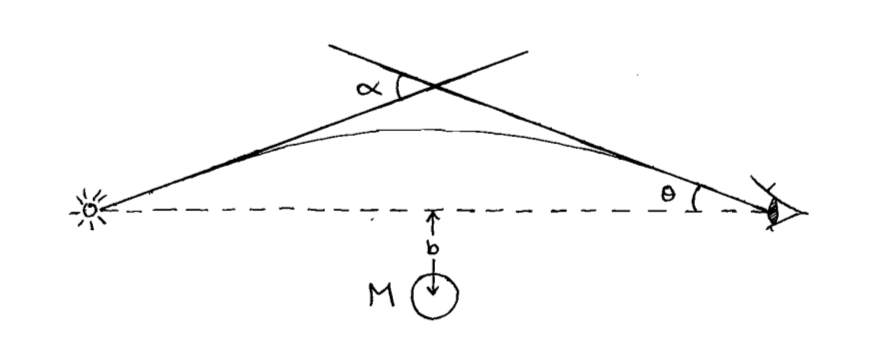
\includegraphics[scale=0.5]{light-bending.png}
\end{center}

yo!

\end{document}